
\documentclass[12pt,openright,twoside,a4paper,article,brazil]{abntex2}

\usepackage[utf8]{inputenc}
\usepackage[T1]{fontenc}
\usepackage{graphicx}
\usepackage{array, tabularx}
\usepackage{rotating}
\usepackage{multirow}
\usepackage{longtable}
\usepackage{listings}
\usepackage{hyperref}
\usepackage{amsmath}
%\usepackage[lofdepth,lotdepth]{subfig}
%\usepackage[alf,abnt-etal-cite=2]{abntex2cite}
\usepackage[num,abnt-etal-cite=2]{abntex2cite}
%\usepackage[num,overcite,abnt-etal-cite=2]{abntex2cite}
\citebrackets[]

\newenvironment{conditions*}
  {\par\vspace{\abovedisplayskip}\noindent
   \tabularx{\columnwidth}{>{$}l<{$} @{\ : } >{\raggedright\arraybackslash}X}}
  {\endtabularx\par\vspace{\belowdisplayskip}}

\graphicspath{{imagens/}}

\titulo{Trabalho de Conclusão da Disciplina Processamento de Linguagem Natural}
%\subtitle{Trabalho de Conclusão da Disciplina Visualização de Dados}
\autor{Vítor Carneiro Curado}
%\subject{Trabalho de Conclusão da Disciplina Visualização de Dados}
\data{\today}
\instituicao{%
	Universidade Federal de Minas Gerais - UFMG
	\par
	Departamento de Ciência da Computação - DCC
	\par
	Programa de Pós-Graduação \emph{Lato Sensu} em Informática
}
\local{Brasília - DF}
\preambulo{Trabalho entregue como requisito para conclusão da disciplina Processamento de Linguagem Natural - programa de pós-graduação \emph{Lato Sensu} em Informática, área de concentração em Gestão de Tecnologia da Informação.}
\orientador{Prof. Dr. Adriano Veloso}

\AtBeginDocument{
	\hypersetup{
		pdftitle={Trabalho de Conclusão da Disciplina Processamento de Linguagem Natural},
		pdfauthor={Vítor Carneiro Curado},
		pdfsubject={\imprimirpreambulo},
		pdfkeywords={Especialização, Tecnologia da Informação, UFMG},
		pdfcreator={LaTeX with abnTeX2}
	}
}

\begin{document}

\frontmatter

%\imprimircapa
%\imprimirfolhaderosto

\maketitle

\tableofcontents

\newpage

\mainmatter



\section{Introdução}
\label{sec:introducao}

O presente trabalho foi desenvolvido como requisito para conclusão da disciplina Processamento de Linguagem Natural, do programa de pós-graduação \emph{Lato Sensu} em Informática, área de concentração em Gestão de Tecnologia da Informação. O objetivo do trabalho é realizar uma avaliação intrínseca de modelos de linguagem neuronais.

Para isso, foi utilizada a ferramenta \emph{word2vec}, que fornece uma implementação das arquiteturas \emph{continuous bag-of-words (CBOW)} and \emph{skip-gram}. A ferramenta em questão está disponível no endereço: \url{https://github.com/tmikolov/word2vec}.

De acordo com as instruções do trabalho prático, a avaliação dos modelos de linguagem deverá variar o tamanho do \emph{corpus}, o tamanho de contexto e, também, a arquitetura CBOW e \mbox{Skip-Gram}.

Considerando o exposto, a seção \ref{sec:metodologia} apresenta a metodologia utilizada na realização do trabalho. Por sua vez, a seção \ref{sec:avaliacao} apresenta a avaliação realizada dos modelos. Por fim, a seção \ref{sec:conclusao} conclui o trabalho.



\section{Metodologia}
\label{sec:metodologia}

A fim de avaliar diferentes modelos de linguagem, foram desenvolvidos dois programas: um \emph{bash script} para criação dos \emph{wordspaces}\footnote{\emph{Wordspace} é um espaço de vetores de palavras.} e um programa em C similar ao \emph{word-analogy}.

O \emph{bash script} teve a finalidade de criar diferentes \emph{wordspaces} variando de forma automatizada o tamanho de contexto, a arquitetura (CBOW e Skip-Gram) e o tamanho do \emph{corpus} utilizado para treinar o modelo. O script em questão está no apêndice \ref{sec:ap-wordspaces}.

O programa em C, por sua vez, teve o propósito de avaliar o \emph{wordspace} criado. Essa avaliação foi realizada utilizando o arquivo \emph{questions-words.txt}. Esse arquivo contem $19.544$ linhas de texto, sendo que cada linha contem 4 palavras. As 3 primeiras palavras são utilizadas pelo programa para tentar calcular o vetor da 4ª palavra, sendo que a 4ª palavra que consta no arquivo \emph{questions-words.txt} é o resultado correto. O erro do modelo, portanto, é calculado com base na distância euclidiana entre a palavra calculada pelo programa e a palavra correta, que consta no arquivo. O código-fonte do programa criado está disponível no apêndice \ref{sec:ap-wordanalogy2}.

Deste modo, foram avaliados \emph{wordspaces} CBOW e Skip-Gram, com tamanho de contexto variando de dois em dois, sendo que o menor contexto avaliado foi de tamanho 2 e o maior foi de tamanho 20. Por sua vez, para treinar o modelo foram utilizados 10 (dez) diferentes tamanhos de \emph{corpus}. Os tamanhos de \emph{corpus} utilizados foram (em quantidade de palavras): $1.650.000$, $3.300.000$, $5.100.000$, $6.750.000$, $8.550.000$, $10.200.000$, $12.000.000$, $13.650.000$, $15.300.000$ e $17.005.207$.

Todos os códigos e arquivos utilizados na realização deste trabalho estão disponíveis para download no endereço:

\url{https://github.com/carneirocurado/Processamento-Linguagem-Natural}

\section{Avaliação dos Modelos}
\label{sec:avaliacao}

A avaliação foi realizada considerando todas as $19.544$ linhas de texto do arquivo  \emph{questions-words.txt}. Para cada linha do arquivo era verificado, em primeiro lugar, se todas as quatro palavras estavam presentes no modelo. Caso alguma dessas quatro palavras não existisse no modelo, essa linha era classificada como \emph{Fora do Dicionário}. Caso, entretanto, todas as quatro palavras estivessem presentes no modelo, os vetores das três primeiras palavras eram utilizados em uma operação algébrica visando encontrar um vetor resultante que tivesse uma relação com o vetor da terceira palavra similar à relação que o vetor da segunda palavra tem com o da primeira.  A equação \ref{eq:vetor-resultante} exemplifica essa operação para o caso de a linha do arquivo ser: \emph{Athens Greece Paris France}.

\begin{equation}
\label{eq:vetor-resultante}
vetor\_resultante =  \left(\overbrace{vetor_2}^{Greece} - \overbrace{vetor_1}^{Athens}\right) + \overbrace{vetor_3}^{Paris}
\end{equation}

Após realizado o cálculo da equação \ref{eq:vetor-resultante}, é esperado que o $vetor\_resultante$ corresponda à palavra \emph{France}, isto é, a palavra \emph{France} deve ser, dentre todas as outras palavras do vocabulário, a mais próxima ao $vetor\_resultante$. Para, então, verificar a acurácia do modelo, é calculada a distância euclidiana entre o $vetor\_resultante$ e todas as outras palavras do vocabulário. Um \emph{ranking}, então, é montado com as $1.000$ (mil) palavras mais próximas do $vetor\_resultante$.  Por fim, é verificada qual a posição da palavra correta (\emph{France}) nesse \emph{ranking}. Caso a palavra \emph{France} esteja fora desse \emph{ranking}, ela é contabilizada como \emph{Fora do Ranking}. Isto é, fora do \emph{ranking} são as palavras que estão no dicionário do modelo mas não estão entre as $1.000$ palavras mais próximas do $vetor\_resultante$. Caso, entretanto, a palavra \emph{France} esteja no \emph{ranking}, o erro do modelo é calculado com base na equação \ref{eq:rmsd}, que calcula a raiz do erro quadrático médio (\emph{Root Mean Squared Deviation} - RMSD) do modelo.

\begin{align}
\label{eq:rmsd}
RMSD =& \sqrt{\frac{\sum_{i=1}^{qtde}\left(d(x) - d(0)\right)^2}{qtde}}
\end{align}

onde:
\begin{conditions*}
qtde & total de linhas analisadas \\
d(x) & distância euclidiana do vetor\_resultante à palavra \emph{France} \\
d(0) & distância euclidiana do vetor\_resultante à palavra mais próxima a ele \\
\end{conditions*}

Conforme pode ser observado pela equação \ref{eq:rmsd}, caso a palavra \emph{France} seja a mais próxima ao $vetor\_resultante$ o erro será zero. O RMSD final do modelo é a raiz do somatório do quadrado do erro de cada linha contabilizada na análise, dividido pelo total de linhas contabilizadas. As linhas contabilizadas são o total de linhas do arquivo \emph{question-words.txt} descontadas as linhas com palavras fora do dicionário ou fora do \emph{ranking}. Cabe destacar que quanto maior o \emph{corpus} utilizado, menor era a quantidade de linhas fora do dicionário. A figura \ref{fig:comparativo-geral} apresenta essa relação. Por sua vez, a quantidade de linhas fora do \emph{ranking} era influenciada pelo tamanho do \emph{corpus}, pelo tamanho do contexto e pela arquitetura do modelo (CBOW ou Skip-Gram). A figura \ref{fig:cbow-ranking} ilustra essa relação para a arquitetura CBOW e a figura \ref{fig:skipgram-ranking} para a Skip-Gram.


\begin{figure}[h]
	\centering
		\makebox[\textwidth]{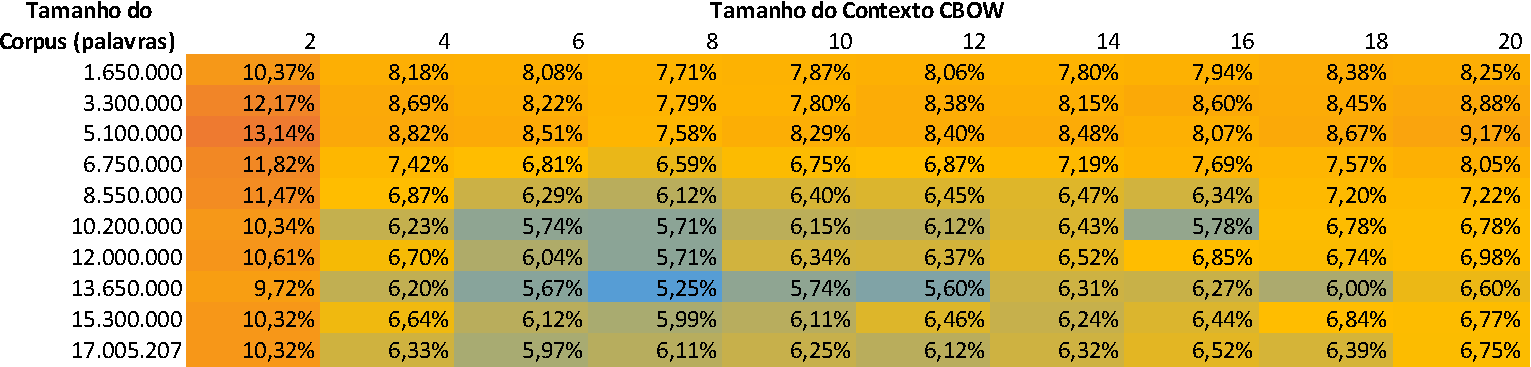
\includegraphics[width=\textwidth]{cbow_ranking.pdf}}
	\caption{Percentual de linhas fora do \emph{ranking} usando o modelo CBOW variando o tamanho do Corpus e o tamanho do Contexto}
	\label{fig:cbow-ranking}
\end{figure}

\begin{figure}[h]
	\centering
		\makebox[\textwidth]{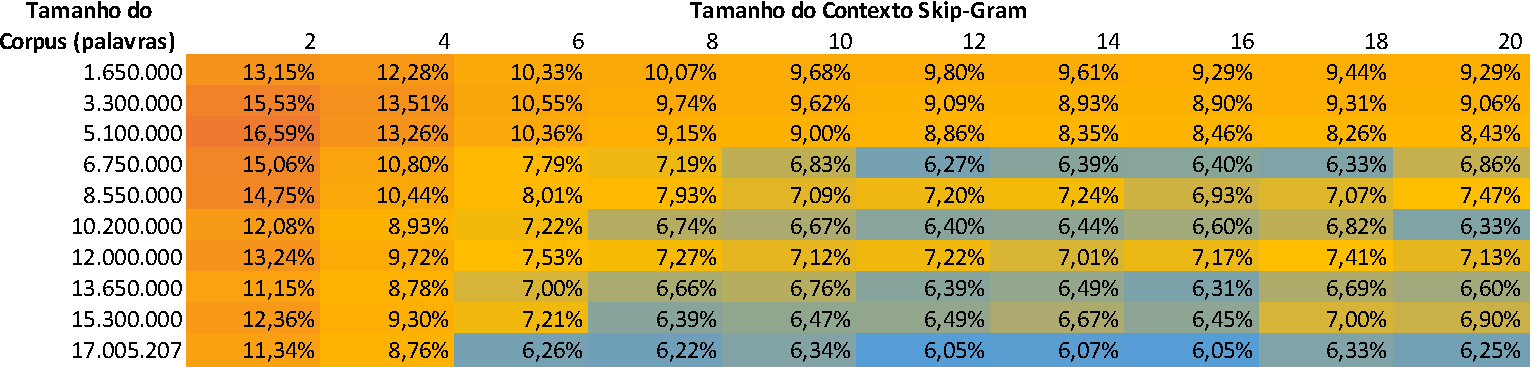
\includegraphics[width=\textwidth]{skipgram_ranking.pdf}}
	\caption{Percentual de linhas fora do \emph{ranking} usando o modelo Skip-gram variando o tamanho do Corpus e o tamanho do Contexto}
	\label{fig:skipgram-ranking}
\end{figure}

Conforme pode ser observado nas figuras \ref{fig:cbow-ranking} e \ref{fig:skipgram-ranking}, aumentar o tamanho do \emph{corpus} sem levar em consideração outros fatores pode levar ao aumento no percentual de linhas classificadas como fora do \emph{ranking}. Para que a análise seja completa, o erro do modelo deve ser considerado. A figura \ref{fig:cbow-rmsd} apresenta a raiz do erro quadrático médio (\emph{Root Mean Squared Deviation} - RMSD) do modelo CBOW e a figura \ref{fig:skipgram-rmsd} apresenta o RMSD para o modelo Skip-Gram. Observando as figuras \ref{fig:cbow-rmsd} e \ref{fig:skipgram-rmsd} é possível notar que o aumento do tamanho do \emph{corpus} sempre diminui o RMSD dos modelos.

\begin{figure}[h]
	\centering
		\makebox[\textwidth]{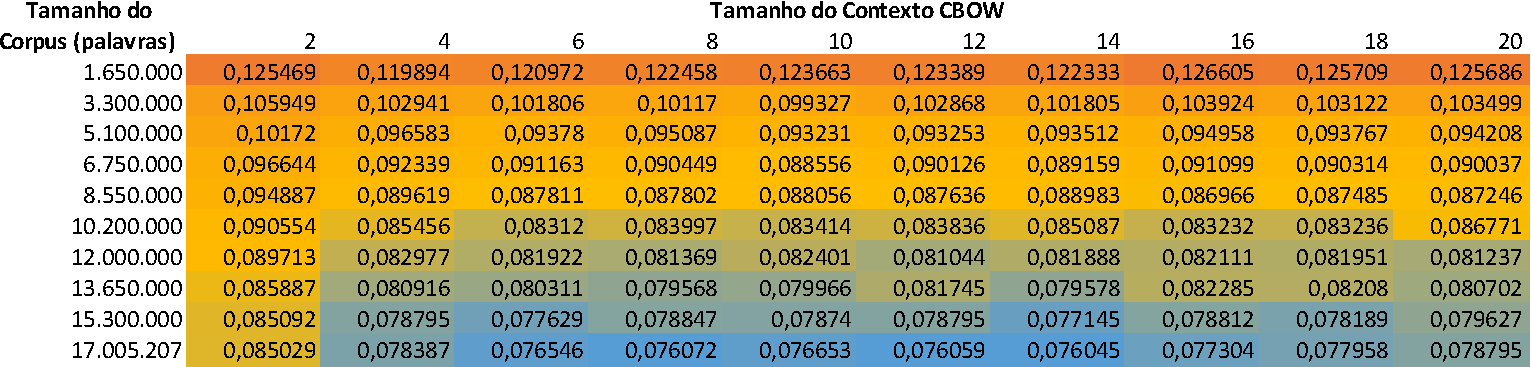
\includegraphics[width=\textwidth]{cbow_rmsd.pdf}}
	\caption{\emph{Root Mean Squared Deviation} do modelo CBOW variando o tamanho do Corpus e o tamanho do Contexto}
	\label{fig:cbow-rmsd}
\end{figure}

\begin{figure}[h]
	\centering
		\makebox[\textwidth]{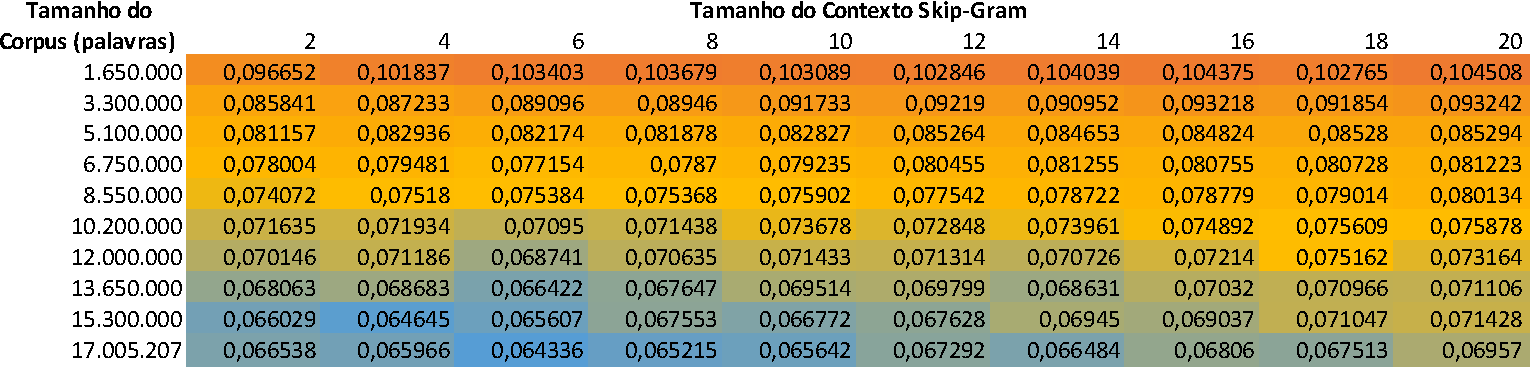
\includegraphics[width=\textwidth]{skipgram_rmsd.pdf}}
	\caption{\emph{Root Mean Squared Deviation} do modelo Skip-gram variando o tamanho do Corpus e o tamanho do Contexto}
	\label{fig:skipgram-rmsd}
\end{figure}

A análise da figura \ref{fig:cbow-rmsd} permite observar que o RMSD mínimo para o modelo CBOW foi de $0,076045$ com um contexto de tamanho $14$. Por sua vez, o RMSD mínimo para o modelo Skip-Gram foi de $0,064336$ com um contexto de tamanho $6$. A figura \ref{fig:comparativo-geral} apresenta o efeito da variação do tamanho do \emph{corpus} com o tamanho de contexto fixo nos melhores valores encontrados para o RMSD.


\begin{figure}[h]
	\centering
		\makebox[\textwidth]{\includegraphics[width=\textwidth]{comparativo-geral.png}}
	\caption{Efeito da variação do tamanho do \emph{corpus} com o tamanho de contexto fixo nos melhores valores encontrados}
	\label{fig:comparativo-geral}
\end{figure}


\section{Conclusão}
\label{sec:conclusao}

O presente trabalho realizou uma avaliação de diferentes modelos de linguagem variando o tamanho do \emph{corpus} utilizado para treinar o modelo, o tamanho de contexto e, também, a arquitetura CBOW e \mbox{Skip-Gram}.

A fim de realizar essa avaliação, foram desenvolvidos dois programas: um \emph{bash script} para criação dos \emph{wordspaces} e um programa em C similar ao \emph{word-analogy}\footnote{Todos os códigos e arquivos utilizados na realização deste trabalho estão disponíveis para download no endereço: \url{https://github.com/carneirocurado/Processamento-Linguagem-Natural}}.

O \emph{bash script} teve a finalidade de criar diferentes \emph{wordspaces} variando de forma automatizada o tamanho de contexto, a arquitetura (CBOW e Skip-Gram) e o tamanho do \emph{corpus} utilizado para treinar o modelo. O programa em C, por sua vez, teve o propósito de avaliar o \emph{wordspace} criado.

Conforme detalhado na seção \ref{sec:avaliacao}, quanto maior era o tamanho do \emph{corpus} utilizado, menor era o percentual de palavras fora do dicionário do modelo. Por sua vez, o percentual de palavras fora do \emph{ranking} era afetado pelo tamanho do \emph{corpus}, pelo tamanho do contexto e pela arquitetura do modelo (CBOW ou Skip-Gram).

Para toda variação de parâmetro foi calculada a raiz do erro quadrático médio (\emph{Root Mean Squared Deviation} - RMSD) do modelo. O menor RMSD para a arquitetura CBOW foi com um contexto de tamanho $14$ e, para a arquitetura Skip-Gram, o menor RMSD foi com um contexto de tamanho $6$. Esses resultados estão detalhados na seção \ref{sec:avaliacao}. A figura \ref{fig:comparativo-geral} ilustra o efeito da variação do tamanho do \emph{corpus} com o tamanho de contexto fixo nesses melhores valores encontrados. Conforme pode ser observado, a arquitetura Skip-Gram foi ligeiramente superior que a CBOW pois, além de apresentar menor erro (RMSD), também apresentou um menor índice de palavras fora do \emph{ranking}. Os modelos que adotavam a arquitetura Skip-Gram, entretanto, foram significativamente mais lentos de se construir que os que adotavam o CBOW.



\backmatter

\postextual

%\pagebreak
\newpage

\bibliography{natural_language_processing}

\apendices

%\pagebreak
\lstset{breaklines=true,numbers=left,extendedchars=true}

\lstset{literate=
  {á}{{\'a}}1 {é}{{\'e}}1 {í}{{\'i}}1 {ó}{{\'o}}1 {ú}{{\'u}}1
  {Á}{{\'A}}1 {É}{{\'E}}1 {Í}{{\'I}}1 {Ó}{{\'O}}1 {Ú}{{\'U}}1
  {à}{{\`a}}1 {è}{{\`e}}1 {ì}{{\`i}}1 {ò}{{\`o}}1 {ù}{{\`u}}1
  {À}{{\`A}}1 {È}{{\'E}}1 {Ì}{{\`I}}1 {Ò}{{\`O}}1 {Ù}{{\`U}}1
  {ä}{{\"a}}1 {ë}{{\"e}}1 {ï}{{\"i}}1 {ö}{{\"o}}1 {ü}{{\"u}}1
  {Ä}{{\"A}}1 {Ë}{{\"E}}1 {Ï}{{\"I}}1 {Ö}{{\"O}}1 {Ü}{{\"U}}1
  {â}{{\^a}}1 {ê}{{\^e}}1 {î}{{\^i}}1 {ô}{{\^o}}1 {û}{{\^u}}1
  {Â}{{\^A}}1 {Ê}{{\^E}}1 {Î}{{\^I}}1 {Ô}{{\^O}}1 {Û}{{\^U}}1
  {œ}{{\oe}}1 {Œ}{{\OE}}1 {æ}{{\ae}}1 {Æ}{{\AE}}1 {ß}{{\ss}}1
  {ű}{{\H{u}}}1 {Ű}{{\H{U}}}1 {ő}{{\H{o}}}1 {Ő}{{\H{O}}}1
  {ç}{{\c c}}1 {Ç}{{\c C}}1 {ø}{{\o}}1 {å}{{\r a}}1 {Å}{{\r A}}1
  {€}{{\euro}}1 {£}{{\pounds}}1 {«}{{\guillemotleft}}1
  {»}{{\guillemotright}}1 {ñ}{{\~n}}1 {Ñ}{{\~N}}1 {¿}{{?`}}1
}

\chapter{Script criação dos Wordspaces}
\label{sec:ap-wordspaces}

\lstinputlisting[language=bash]{../codigo/word-analogy2.sh}

\chapter{Código-fonte}
\label{sec:ap-wordanalogy2}

\lstinputlisting[language=C]{../codigo/word-analogy2.c}



\end{document}
